\documentclass[12pt]{article}
\usepackage{amsmath}
\usepackage{amssymb}
\usepackage{cancel}
\usepackage{enumitem}
\usepackage{esdiff}
\usepackage{graphicx}
\usepackage{siunitx}
% \usepackage{pgfplots}
\usepackage{wrapfig}

\newcommand{\E}[1]{\times 10^{#1}}

\title{
    Worksheet \#8
    \\  \small
    PHYS 4C: Waves and Thermodynamics
    }
\author{Donald Aingworth IV}
\date{October 20, 2025}

\begin{document}
    \DeclareSIUnit{\celsiusdegree}{C^\circ}
    \DeclareSIUnit{\atm}{ atm}

    \maketitle

    \setcounter{section}{0}
    \section{Problem 1}
        The speed of sound in steel is 5941\,\unit{\meter/\second}.
        Steel has a density of around 7900\,\unit{\kilo\gram/\meter^3} (depends somewhat on the alloy content).
        
        a. Based on this information, what is the bulk modulus of steel?

        \begin{wrapfigure}{r}{0.25\textwidth}
            % \vspace{-30pt}
            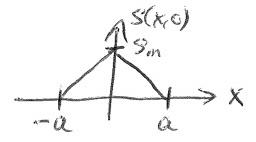
\includegraphics[width=0.25\textwidth]{4c-wspic-1617B.jpg} 
        Sound pulse graph
            % \label{fig:wrapfig}
        \end{wrapfigure}
        b. A steel rod of cross-sectional area A is placed on the x-axis.  
        The following sound pulse is sent through the steel rod in the +x direction:
        
        $f(x) = s(x,0) = s_m(1 - |x|/a)$, if $|x| < a$.
        
        $f(x) = s(x,0) = 0$, if $|x| \geq a$.

        % 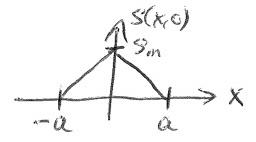
\includegraphics{4c-wspic-1617B.jpg}
        
        Determine the total energy of this pulse.
        
        c. Now suppose a sinusoidal sound wave with frequency $440\,\unit{\hertz}$ is sent through steel with a sound level of $100\,\unit{\deci\bel}$.  
        Calculate $s_m$ and $\Delta p_m$ for this sound wave.

        \subsection{Solution (a)}
            The bulk modulus is used as part of an equation for the velocity.
            \begin{equation}
                v   =   \sqrt{\frac{B}{\rho}}
            \end{equation}

            This can be solved for the bulk modulus.
            \begin{equation}
                B   =   \rho v^2
            \end{equation}

            We know all the values necessary, so we can solve this equation.
            \begin{equation}
                B   =   (7900\,\unit{\kilo\gram/\meter^3}) (5941\,\unit{\meter/\second})^2
                    =   \boxed{2.788\E{11}\,\unit{\kilo\gram/\meter\cdot\second^2}}
            \end{equation}
        
        \subsection{Solution (b)}
            First, using the equations of $f(x)$, we can 
            
        
    \section{Problem 2}
        A half-open organ pipe is tuned to A(440) (i.e., the fundamental frequency is $440\,\unit{\hertz}$).
        Air has a density of $1.21\,\unit{\kilo\gram/\mole}$ and a speed of sound of $343\,\unit{\meter/\second}$ at $20\unit{\celsius}$.
        
        \begin{enumerate}[label=\alph*.]
            \item   What is the length of the pipe?
            \item   What is the maximum kinetic energy density (per unit volume) at the open end of the pipe if $s_m = 2.0\,\unit{\micro\meter}$?  At the closed end?
            \item   If the ambient temperature were raised from 20\unit{\celsius} to 40\unit{\celsius}, what would be the new fundamental frequency of the pipe (ignore changes in the length of the pipe due to the temperature change)?
        \end{enumerate}
    




\end{document}